%%%%%%%%%%%%%%%%%%%%%%%%%%%%%%%%%%%%%%%%%%%%%%%%%%%%%%%%%%%%%%%%%%%%%

\documentclass[11pt,aspectratio=169]{beamer}

\def\lingua{gal}

\def\nome{Queijo Seoane, Daniel}
\def\nomedirectorA{Padrón González, Emilio José}
\def\nomedirectorB{Vázquez Araújo, Francisco Javier}

\def\titulo{Emulador de GameBoy para sistemas embebidos}
\def\titulocurto{Emulador de GameBoy para sistemas embebidos}
\def\titulacion{gei}
\def\mencion{ENXEÑARÍA DE COMPUTADORES}

\usepackage{estilo_defensa}


\usepackage{multirow}
\usepackage{pgfgantt}

% os diagramas TikZ tómanse da memoria, que usa o paquete glossaries;
% aquí abonda con expandir os acrónimos a maiúsculas
\providecommand{\acrshort}[1]{\MakeUppercase{#1}}
\providecommand{\acrshortpl}[1]{\MakeUppercase{#1}s}
\providecommand{\acrlong}[1]{#1}
\providecommand{\acrfull}[1]{\MakeUppercase{#1}}
\usetikzlibrary{positioning, fit, arrows.meta, backgrounds, shapes.multipart, shapes.geometric, calc}

% definición da linguaxe Rust para listings, tomada de https://github.com/denki/listings-rust (licenza BSD 3-Clause)
\usepackage{listings-rust}
\lstset{
  keywordstyle=[2]\color{udcpink},
  keywordstyle=[3]\color{udcpink},
  keywordstyle=[4]\color{udcpink},
  keywordstyle=[5]\color{ficblue}\itshape
}

%%% METADATOS DA PRESENTACIÓN %%%
\title[\titulocurto]{\titulo}
\author[\nome]{\nome}
\date{\datasimple}
\titlegraphic{}


\begin{document}



 %%%%%%%%%%%%%%%%%%%%%%%%%%%%%%%%%%%%%%%%%%%%%%%%%%%%%%%%%%%%%%%%%%%%%%%%%%%%%%%%
% Portada da defensa                                                           %
% Réplica da portada da memoria (portada/portada.tex) adaptada a formato 16:9.  %
% Os datos (nome, título, dirección, titulación) tómanse de defensa_tfg.tex.    %
%%%%%%%%%%%%%%%%%%%%%%%%%%%%%%%%%%%%%%%%%%%%%%%%%%%%%%%%%%%%%%%%%%%%%%%%%%%%%%%%

\begin{frame}[plain,noframenumbering]

  \textcolor{udcpink}{{\fontencoding{T1}\fontfamily{phv}\selectfont\footnotesize Facultade de Informática}}

  \vspace{0.2cm}

  \begin{center}
    % logos oficiais: selo da UDC e selo EURO-INF (este último, só no GEI)
    \begin{minipage}[c]{0.46\textwidth}
      \raggedleft
\includegraphics[width=0.72\textwidth]{imaxes/udc}
    \end{minipage}%
    \hspace{0.04\textwidth}%
    \begin{minipage}[c]{0.20\textwidth}
      \raggedright\carimbo
    \end{minipage}

    \vspace{0.35cm}

    {\scriptsize\color{udcgray}
      \nometfg \\
      \nometitulacion \\
      \nomemencion }

    \vspace{0.45cm}

    {\color{udcpink}\rule{0.5\paperwidth}{0.5mm}}

    \vspace{0.35cm}

    {\usebeamerfont{title}\usebeamercolor[fg]{title}\titulo\par}
  \end{center}

  \vfill

  \begin{flushright}
    {\small
    \begin{tabular}{ll}
      {\bf \nomeestudante:} & \nome \\
      {\bf \nomedirixe:}    & \nomedirectorA \\
                            & \nomedirectorB \\ % duplica esta liña se o precisas, cambiando
                                                % a letra final (A, B, C...); defínense en defensa_tfg.tex
    \end{tabular}}
  \end{flushright}

  \rightline{{\small\color{udcgray}A Coruña, \datasimple.}}

\end{frame}


 \begin{frame}{\nomeindice}
   \tableofcontents
 \end{frame}

 \section{Introdución}

\begin{frame}{Contexto e motivación}
  \begin{itemize}
    \item Primeira idea por desenvolver
    \item Segunda idea por desenvolver
    \begin{itemize}
      \item Subpunto por desenvolver
    \end{itemize}
  \end{itemize}
\end{frame}

\begin{frame}{Obxectivos}
  \begin{block}{Obxectivo principal}
    Enunciado por desenvolver.
  \end{block}

  \vspace{0.5em}

  \begin{itemize}
    \item Obxectivo específico por desenvolver
    \item Obxectivo específico por desenvolver
  \end{itemize}
\end{frame}

 \section{Metodoloxía e planificación}

\begin{frame}{Desenvolvemento iterativo e incremental}
  \begin{columns}[c]
    \begin{column}{0.42\textwidth}
      \small
      \begin{itemize}
        \item Once iteracións, onde a maioría corresponde cun
        compoñente do hardware da Game Boy.

        \item A orde vén imposta polo acoplamento do hardware.

        \item O desenvolvemento dos compoñenetes segue unha estrutura de estudo da arquitectura, implementación
          e validación.

        \item Git e GitHub, empregando \textit{conventional commits} e \textit{conventional branch}
        para manter un historial de cambios limpo.

      \end{itemize}
    \end{column}
    \begin{column}{0.56\textwidth}
      \begin{center}
      \begin{ganttchart}[
          hgrid, vgrid,
          x unit=0.38cm,
          y unit title=0.40cm,
          y unit chart=0.32cm,
          title height=1,
          title label font=\tiny\bfseries,
          bar/.style={fill=udcpink!75, draw=udcpink!90},
          bar height=0.62,
          bar label font=\tiny,
        ]{1}{18}
        \gantttitle{2025}{6}\gantttitle{2026}{12} \\
        \gantttitle{O}{2}\gantttitle{N}{2}\gantttitle{D}{2}
        \gantttitle{X}{2}\gantttitle{F}{2}\gantttitle{M}{2}
        \gantttitle{A}{2}\gantttitle{M}{2}\gantttitle{X}{2} \\
        \ganttbar{It. 1}{1}{1} \\
        \ganttbar{It. 2}{1}{2} \\
        \ganttbar{It. 3}{2}{5} \\
        \ganttbar{It. 4}{4}{6}\ganttbar{It. 4}{9}{9} \\
        \ganttbar{It. 5}{3}{6} \\
        \ganttbar{It. 6}{9}{10} \\
        \ganttbar{It. 7}{10}{11} \\
        \ganttbar{It. 8}{11}{13} \\
        \ganttbar{It. 9}{12}{13} \\
        \ganttbar{It. 10}{14}{15} \\
        \ganttbar{It. 11}{15}{16} \\
        \ganttbar[bar/.append style={fill=udcgray!50, draw=udcgray}]{Doc.}{15}{18}
      \end{ganttchart}\\[0.4em]
      \fonte{Diagrama de Gantt do proxecto.}
      \end{center}
    \end{column}
  \end{columns}
\end{frame}

 \section{Ferramentas e tecnoloxías}

\begin{frame}{Linguaxe, librería e manexador de paquetes}
  \vfill
  \begin{itemize}
    \setlength{\itemsep}{1.6em}

    \item \destacado{Rust}: unha linguaxe de programación de sistemas. Compilado, fortemente tipado
    e con manexo automático de memoria sen \textit{garbage collector}.

    \item \destacado{Raylib}: librería para o desenvolvemento de videoxogos, coa que se manexa vídeo, audio e entrada de forma sinxela,
    puidendo compilarse para todo tipo de plataformas.

    \item \destacado{Nix}: manexador de paquetes declarativo,
    que permite definir contornas de desenvolvemento e imaxes completas dun sistema embebido de forma reproducibles.
  
  \end{itemize}
  \vfill
\end{frame}

\begin{frame}[plain,noframenumbering]{Anexo · Arquitectura de raylib}
  \begin{center}
    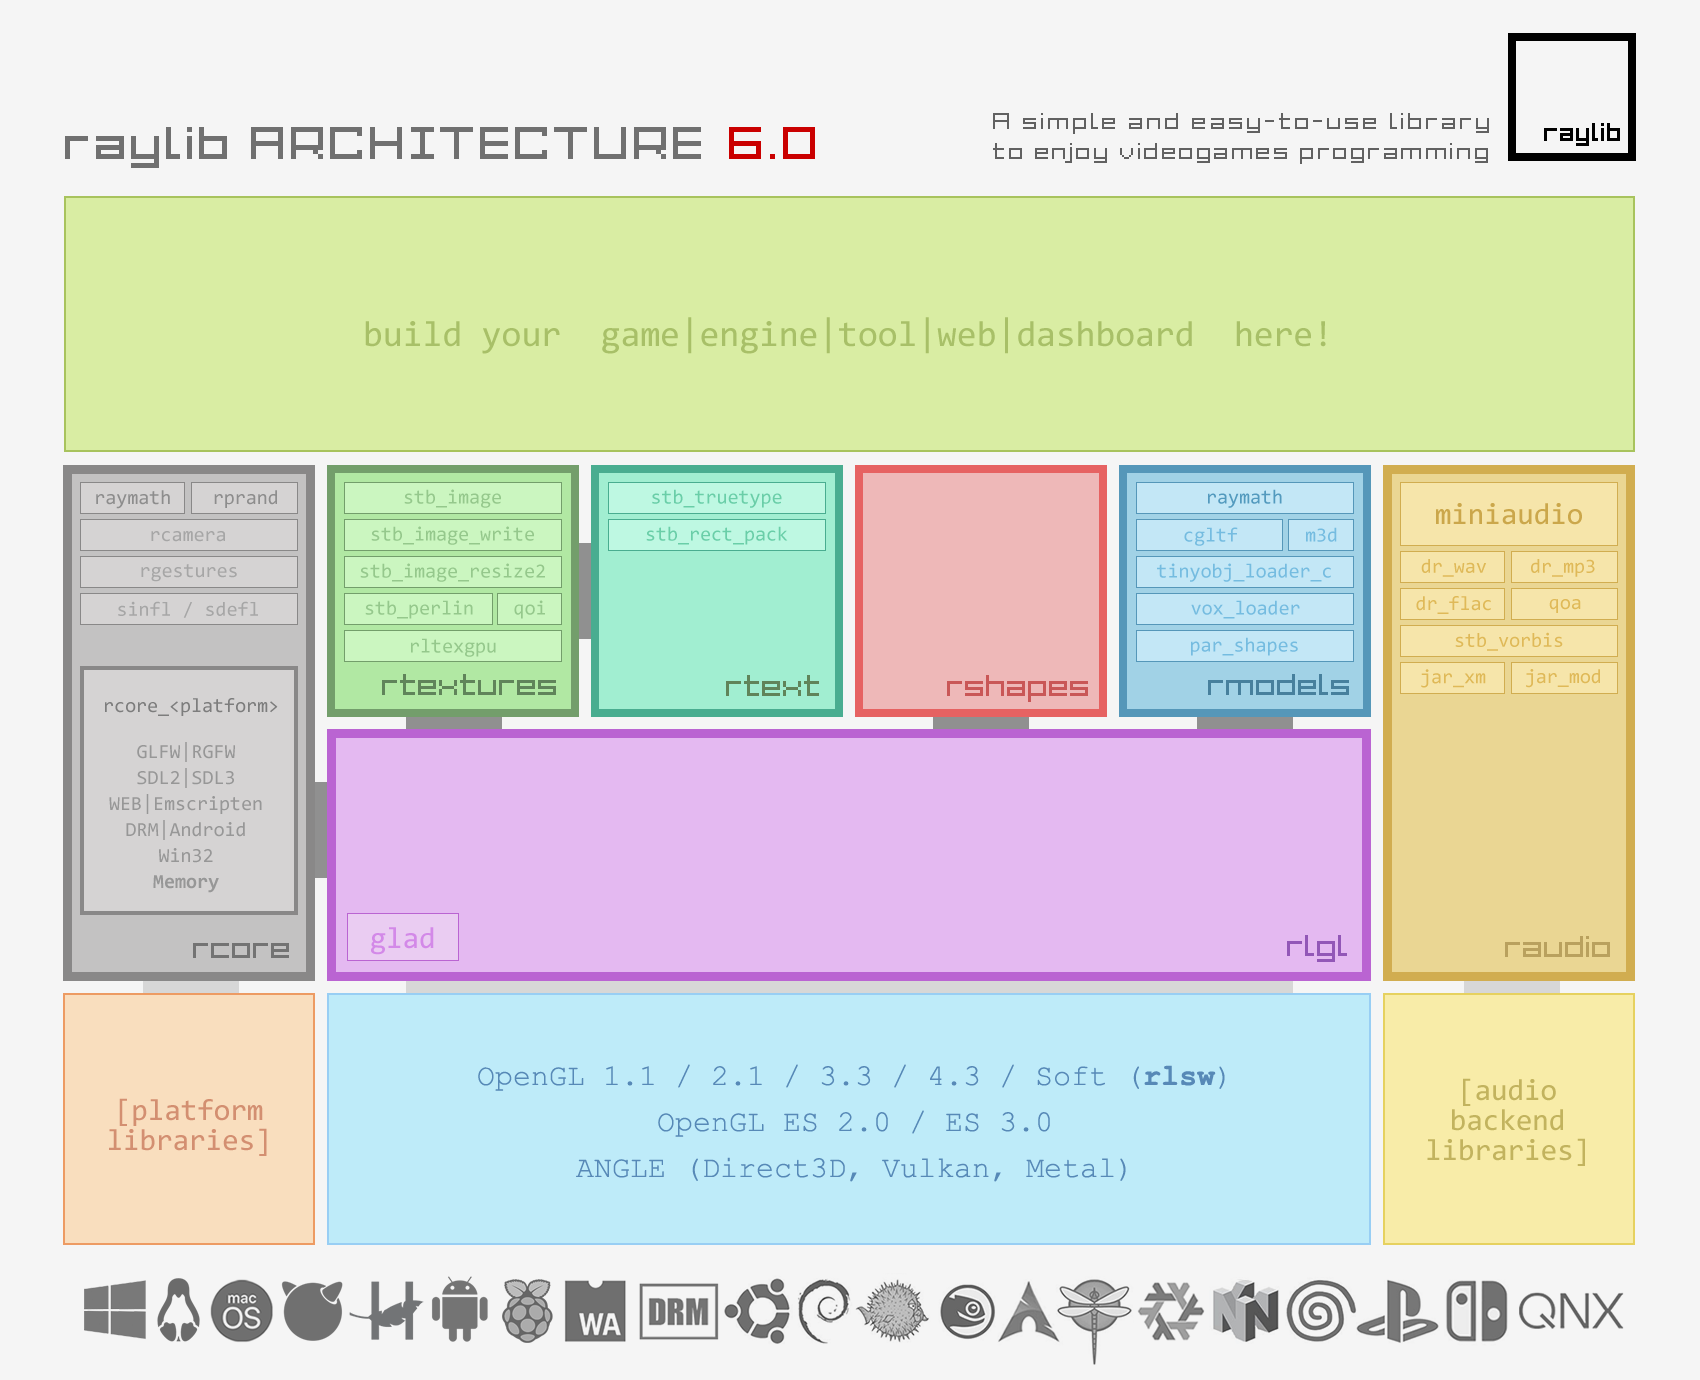
\includegraphics[height=0.78\textheight,keepaspectratio]{imaxes/raylib_architecture_v6.0.png}
  \end{center}
\end{frame}

 \section{Arquitectura}

\begin{frame}{Arquitectura do sistema}
  \imaxe[0.62\textwidth]{imaxes/arch_diagram.png}{Diagrama da arquitectura da Game Boy}
\end{frame}

\begin{frame}{Mapa de memoria}
  \begin{columns}[c]
    \begin{column}{0.46\textwidth}
      \begin{itemize}
        \item Idea por desenvolver
        \item Idea por desenvolver
      \end{itemize}
    \end{column}
    \begin{column}{0.46\textwidth}
      \imaxe[0.72\textwidth]{imaxes/memory_map.png}{Mapa de memoria}
    \end{column}
  \end{columns}
\end{frame}

 
\begin{frame}{Un paso do procesador}
  \begin{columns}[c]
    \begin{column}{0.36\textwidth}
      \small
      \begin{itemize}
        \item Primeiro \destacado{aténdese ás interrupcións} pendentes segundo a súa prioridade.
        \item Se non as hai, búscase, decodifícase e execútase a instrución.
        \item O tempo consumido é o que despois fai avanzar
          \textsc{ppu}, \textsc{apu}, temporizadores e porto serie.
      \end{itemize}
    \end{column}
    \begin{column}{0.62\textwidth}
      \begin{center}

        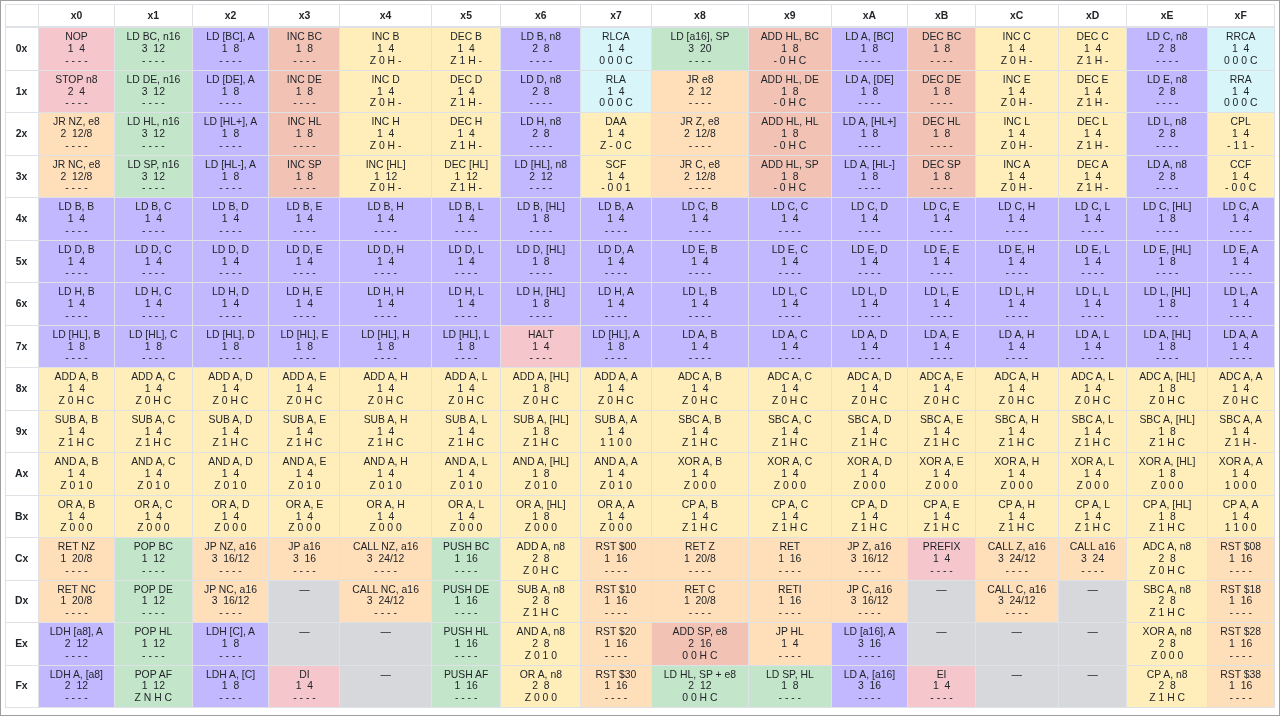
\includegraphics[width=\textwidth,height=0.74\textheight,keepaspectratio]{imaxes/sm83_instruction_set.png}\\[0.3em]
        \fonte{Táboa principal de \textit{opcodes}.}

      \end{center}
    \end{column}
  \end{columns}
\end{frame}

\begin{frame}{Execución dunha instrución}
  \vfill
  \begin{itemize}
    \setlength{\itemsep}{1.1em}
    \item Unha instrución é un \texttt{struct} que implementa
      \texttt{Instruction} e o operando é un \destacado{parámetro xenérico}
      que xa sabe o seu tamaño e o seu custo en ciclos.
    \item \texttt{exec} le o operando fonte, escribe no destino e devolve o
      efecto da instrución.
    \item \texttt{InstructionEffect} devolve o tempo consumido e as
      bandeiras: cada unha pode quedar a \texttt{true}, a \texttt{false} ou
      \destacado{sen cambios}.
    \item \texttt{info} resólvese a partir das constantes asociadas dos
      operandos, \destacado{en tempo de compilación}.
    \item Un módulo por instrución, sen código repetido e sen custo
      en tempo de execución.
  \end{itemize}
  \vfill
\end{frame}

\begin{frame}[fragile]{Execución dunha instrución}
\begin{lstlisting}[language=Rust,basicstyle=\ttfamily\fontsize{7.8pt}{8.3pt}\selectfont,breaklines=false]
pub struct Ld<D: WritableOperand, S: Operand> {
  dst: D,
  src: S,
}
impl<D: WritableOperand, S: Operand> Ld<D, S> {
  pub fn new(dst: D, src: S) -> Self { Self { dst, src } }
}
impl<D: WritableOperand, S: Operand> Instruction for Ld<D, S> {
  fn exec(&mut self, gb: &mut Dmg) -> InstructionResult {
    let value = self.src.read(gb);
    self.dst.write(gb, value);

    Ok(InstructionEffect::new(self.info(), Flags::none()))
  }
  fn info(&self) -> (u8, u8) {
    (1 + S::READ_CYCLES + D::WRITE_CYCLES, 1 + S::LEN + D::LEN)
  }
  fn disassembly(&self) -> String {
    format!("ld {},{}", self.dst, self.src)
  }
}
\end{lstlisting}
\end{frame}



\begin{frame}{Unidade de procesamento de píxeles}
  \begin{columns}[c]
    \begin{column}{0.44\textwidth}
      \small
      \begin{itemize}
        \item Unha máquina de estados percorre os modos da \textsc{ppu}:
        \texttt{OAM search}, \texttt{pixel transfer}, \texttt{HBlank} e \texttt{VBlank}.
        
        \item \textit{scanline rendering} debuxa cada liña con \texttt{draw\_bg}, \texttt{draw\_window} e \texttt{draw\_sprites},
        de esquerda a dereita resolvendo prioridades e transparencia.
        
        \item O fondo garda unha \destacado{caché de identificadores de cor}
        coa que despois se resolven as prioridades dos obxectos facilmente.

      \end{itemize}
    \end{column}
    \begin{column}{0.54\textwidth}
      \imaxe[\textwidth]{imaxes/ppu_composition.png}{Composición dun cadro: fondo, xanela e obxectos.}
    \end{column}
  \end{columns}
\end{frame}


\begin{frame}[plain,noframenumbering]
  \begin{center}
    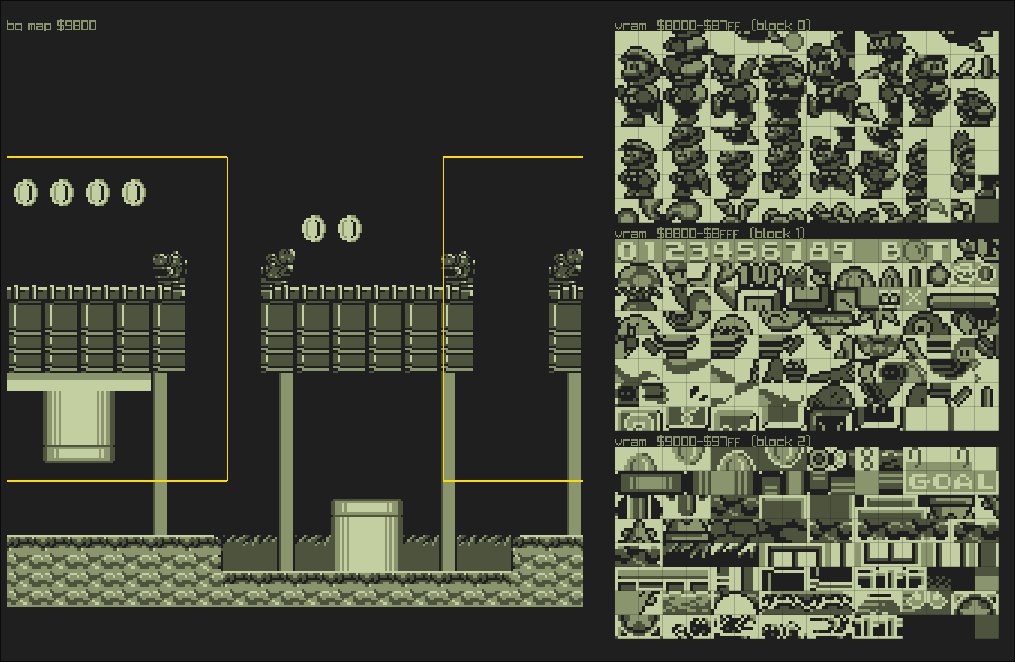
\includegraphics[width=0.84\textwidth,height=0.76\textheight,keepaspectratio]{imaxes/vram_oam_representation.png}\\[0.4em]
    \fonte{Ferramentas de depuración: contido da \textsc{vram} e dos obxectos da \textsc{oam}.}
  \end{center}
\end{frame}

\begin{frame}{Os cartuchos amplían o hardware da consola}
  \vfill
  \begin{itemize}
    \setlength{\itemsep}{1.4em}

    \item A Game Boy emprega os cartuchos para engadir hardware adicional
    A configuración deste hardware faise mediante escrituras no espazo de direccións da \textsc{rom}.

    \item O \textsc{mbc} encárgase de xestionar ese hardware. Existen moitos,
    dos que se implementaron os cinco máis habituais: sen \textsc{mbc},
    \textsc{mbc}1, \textsc{mbc}2, \textsc{mbc}3 e \textsc{mbc}5.

    \item O seu cometido principal é \destacado{intercambiar os bancos de
    \textsc{rom} e \textsc{ram}} para aumentar a memoria dispoñible.

  \end{itemize}
  \vfill
\end{frame}

\begin{frame}[fragile]{Os cartuchos amplían o hardware da consola}
\begin{lstlisting}[language=Rust,breaklines=false]
fn write_rom(&mut self, address: u16, value: u8) {
  match address {
    RAM_AND_TIMER_ENABLE_START..=RAM_AND_TIMER_ENABLE_END => {
      let enabled = (value & 0x0F) == 0x0A;
      ...
    }

    ROM_BANK_NUMBER_START..=ROM_BANK_NUMBER_END => {
      self.rom_selected_bank = value & 0x7F;
    }

    RAM_BANK_NUMBER_OR_RTC_SELECT_START..=RAM_BANK_NUMBER_OR_RTC_SELECT_END => {
      if value <= 0x03 {
        self.ram_selected_bank = value;
        self.rtc_selected = false;
        ...
\end{lstlisting}
\end{frame}

\begin{frame}{Optimización}
  \begin{columns}[c]
    \begin{column}{0.46\textwidth}
      \small
      \begin{itemize}
        \item \destacado{Bucles de debuxado}: reutilizar cálculos entre píxeles
        consecutivos e acceso directo ás memorias da \textsc{ppu}.

        \item \destacado{Complexidade}: temporizador e \textsc{apu} son
        contadores periódicos; en vez de iterar nun bucle segundo o tempo avanzado pola \textsc{cpu},
        % calculase canto tempo falta para o seguinte evento e avánzase directamente.

        \item \destacado{Bucle quente}: elimminouse o uso de memoria no \textit{heap} no bucle quente
        e o \textit{dynamic dispatching} substituíuse por resolución estática e monomorfización.
      \end{itemize}
    \end{column}
    \begin{column}{0.52\textwidth}
      \begin{center}
        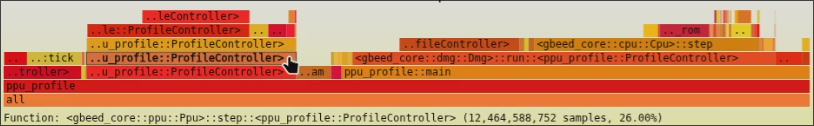
\includegraphics[width=\textwidth]{imaxes/flamegraph_baseline.png}\\[0.2em]
        \fonte{Antes: o debuxado supón o 26,0\,\% do tempo.}\\[0.7em]
        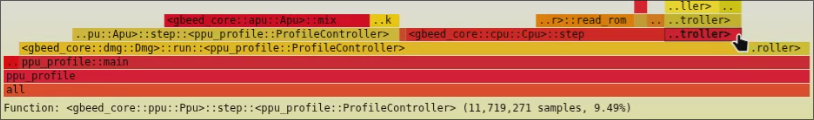
\includegraphics[width=\textwidth]{imaxes/flamegraph_optimized.png}\\[0.2em]
        \fonte{Despois: 9,5\,\%.}
      \end{center}
    \end{column}
  \end{columns}
\end{frame}

\begin{frame}{Dúas interfaces sobre o mesmo núcleo}
  \vfill
  \begin{block}{Interface de depuración}
    Amosa o estado da \textsc{vram} e a entrada do mando. % moi util para comprobar erro
    Compilada a WebAssembly con Emscripten e despregada en GitHub Pages
    con cada confirmación.
  \end{block}
  \vspace{1em}
  \begin{block}{Interface de estilo consola}
    Consegue unha experiencia de usuario similar á unha consola.
    Incorpora menús para o control do emulador e varias características de calidade de vida
  \end{block}
  \vfill
\end{frame}

\begin{frame}{Do emulador á consola}
  \begin{columns}[c]
    \begin{column}{0.46\textwidth}
      \small
      \begin{itemize}

        \item \destacado{Raspberry Pi Zero W} (\texttt{armv6l}) e
        \destacado{Zero 2 W} (\texttt{aarch64}).

        \item \destacado{GamePi13}: pantalla \textsc{IPS} con controlador
        ST7789, altofalante e botóns, conectado aos \textsc{gpio} \textbf{sen soldadura}.

      \end{itemize}
    \end{column}
    \begin{column}{0.52\textwidth}
      \imaxe[\textwidth]{imaxes/gamepi13.png}{A construción de referencia executando o emulador.}
    \end{column}
  \end{columns}
\end{frame}

\begin{frame}{Unha imaxe de sistema reproducible}
  \footnotesize
  \begin{columns}[t]
    \begin{column}{0.49\textwidth}
      \begin{block}{NixOS en RPi Zero 2 W}
        \begin{itemize}
          \item A pantalla emprégase co controlador \texttt{panel-mipi-dbi},
          en vez de usar o \textit{stack} obsoleto documentado polo fabricante.

          \item O \textit{firmware} de inicialización do ST7789V e o
          \textit{overlay} do audio por \textsc{pwm} xéranse en tempo de evaluación,
          sen configuración manual requerida.

          \item Emprégase o núcleo \texttt{drm} de Raylib sen unha sesión gráfica completa. 

          \item Unha imaxe de \textsc{sd} lista para gravar que arranca o emulador directamente,

        \end{itemize}
      \end{block}
    \end{column}
    \begin{column}{0.49\textwidth}
      \begin{block}{Debian do fabricante en RPi Zero W}
        \begin{itemize}
          \item \texttt{armv6l} non está soportada por NixOS polo que o mellor é partir da imaxe preconfigurada do fabricante.

          \item \textit{fbcp} copia o \textit{framebuffer} principal a través de DispmanX
          e só funciona sobre X11.

          \item \destacado{Materializouse un dos riscos previstos}. Obrigou a
          cambiar o backend \textsc{drm} polo de X11.

          \item O binario obtense por compilación cruzada nun contedor.
        \end{itemize}
      \end{block}
    \end{column}
  \end{columns}
\end{frame}

\begin{frame}[fragile]{Unha imaxe de sistema reproducible}
\begin{lstlisting}[language=Nix,breaklines=false]
{
  inputs,
  outputs,
  ...
}: {
  gbeed02 = inputs.nixpkgs-pi.lib.nixosSystem {
    specialArgs = {
      inherit inputs outputs;
      hostname = "gbeed02";
      username = "gbeed";
    };
    modules = [
      "${inputs.nixpkgs-pi}/nixos/modules/installer/sd-card/sd-image-aarch64.nix"
      ./gbeed02/configuration.nix
      ./gbeed02/hardware-configuration.nix
    ];
  };
}
\end{lstlisting}
\end{frame}

 \section{Probas e validación}

\begin{frame}{Tres niveis de validación}
  \begin{columns}[c]
    \begin{column}{0.56\textwidth}
      \footnotesize
      \begin{itemize}
        \item \destacado{Probas unitarias} sobre as instrucións máis complexas
        da \textsc{cpu}.

        \item \destacado{Suites de referencia da comunidade}, validadas en hardware real:
          \begin{itemize}
            \item \texttt{blargg}: \texttt{cpu\_instrs}, \texttt{instr\_timing} e \texttt{dmg\_sound}.
            \item \texttt{mooneye}: controladores de bancos de memoria.
            \item \texttt{dmg-acid2}: a unidade gráfica.
          \end{itemize}

        \item \destacado{Xogos comerciais}: probáronse os máis destacados da plataforma.

      \end{itemize}
    \end{column}
    \begin{column}{0.42\textwidth}
      \imaxe[0.9\textwidth]{imaxes/dmg_acid2.png}{Proba dmg-acid2 superada.}
    \end{column}
  \end{columns}
\end{frame}

\begin{frame}{Validación con xogos comerciais}
  \begin{center}
    {\footnotesize
    \rowcolors{2}{white}{udcgray!20}%
    \begin{tabular}{l|l|c|c|l}
      \rowcolor{udcpink!25}
      \textbf{Xogo} & \textbf{Cartucho} & \textbf{\textsc{rom}} & \textbf{\textsc{ram}} & \textbf{Estado} \\\hline
      Pokémon Red        & MBC3 + \textsc{ram} + batería                  & 1\,MiB   & 32\,KiB & Xogable \\
      Tetris             & Sen controlador                                 & 32\,KiB  & ---     & Xogable \\
      Pokémon Gold       & MBC3 + \textsc{rtc} + \textsc{ram} + batería    & 2\,MiB   & 32\,KiB & Xogable \\
      Pokémon Crystal    & MBC3 + \textsc{rtc} + \textsc{ram} + batería    & 2\,MiB   & 32\,KiB & Non compatible \\
      Super Mario Land   & MBC1                                            & 64\,KiB  & ---     & Xogable \\
      Super Mario Land 2 & MBC1 + \textsc{ram} + batería                   & 512\,KiB & 8\,KiB  & Xogable \\
      Pokémon Pinball    & MBC5 + vibración + \textsc{ram} + batería       & 1\,MiB   & 8\,KiB  & Xogable \\
      Link's Awakening   & MBC1 + \textsc{ram} + batería                   & 512\,KiB & 8\,KiB  & Xogable \\
    \end{tabular}}\\[0.4em]
    \fonte{Os xogos máis vendidos do catálogo, escollidos para cubrir todos os tipos de cartucho implementados.}
  \end{center}
\end{frame}

 \section{Demostración}

% \begin{frame}[plain,noframenumbering]
%   \vfill
%   \begin{center}
%     {\color{ficblue}\Huge\bfseries O emulador na construción de referencia}\\[0.6em]
%     {\color{udcpink}\rule{0.35\paperwidth}{0.5mm}}\\[0.8em]
%     {\large\color{udcgray}Demostración}
%   \end{center}
%   \vfill
% \end{frame}

 \section{Conclusións}

\begin{frame}{Conclusións}
  \begin{itemize}
    \item Conclusión por desenvolver
    \item Conclusión por desenvolver
  \end{itemize}
\end{frame}

\begin{frame}{Traballo futuro}
  \begin{itemize}
    \item Liña de traballo por desenvolver
    \item Liña de traballo por desenvolver
  \end{itemize}
\end{frame}



 %%%%%%%%%%%%%%%%%%%%%%%%%%%%%%%%%%%%%%%%%%%%%%%%%%%%%%%%%%%%%%%%%%%%%%%%%%%%%%%%
% Diapositiva de peche                                                         %
%%%%%%%%%%%%%%%%%%%%%%%%%%%%%%%%%%%%%%%%%%%%%%%%%%%%%%%%%%%%%%%%%%%%%%%%%%%%%%%%

\begin{frame}[plain,noframenumbering]
  \vfill
  \begin{center}
    {\color{ficblue}\Huge\bfseries Grazas pola vosa atención}\\[0.6em]
    {\color{udcpink}\rule{0.3\paperwidth}{0.5mm}}\\[0.8em]
    {\small\color{udcgray}\nome}
  \end{center}
  \vfill
\end{frame}

%  \begin{frame}[plain,noframenumbering]{Material de apoio}
  \begin{itemize}
    \item Diapositiva de apoio por desenvolver
  \end{itemize}
\end{frame}


\end{document}

